\section{ロジスティック回帰とパーセプトロン}
logistic regression, perceptron
1層パーセプトロン
\url{https://www.cs.utexas.edu/~gdurrett/courses/fa2022/perc-lr-connections.pdf}
add SyntheticDatasets
よりも正規分布×2の方がいいか
\url{https://en.wikipedia.org/wiki/Perceptron}

\url{https://arxiv.org/abs/2012.03642}


perceptronは0/1 or -1/1のどちらか

UNDERSTANDING STRAIGHT-THROUGH ESTIMATOR IN TRAINING ACTIVATION QUANTIZED NEURAL NETS

Yoshua Bengio, Nicholas L´eonard, and Aaron Courville. Estimating or propagating gradients through stochastic neurons for conditional computation. arXiv preprint arXiv:1308.3432, 2013.

Hinton (2012) in his lecture 15b

G. Hinton. Neural networks for machine learning, 2012.
\url{https://www.cs.toronto.edu/~hinton/coursera_lectures.html}

delta rule
\lstinputlisting[language=julia]{./text/local-learning-rule/logistic-regression-perceptron/003.jl}
\lstinputlisting[language=julia]{./text/local-learning-rule/logistic-regression-perceptron/004.jl}
\lstinputlisting[language=julia]{./text/local-learning-rule/logistic-regression-perceptron/005.jl}
\lstinputlisting[language=julia]{./text/local-learning-rule/logistic-regression-perceptron/006.jl}
\begin{figure}[ht]
	\centering
	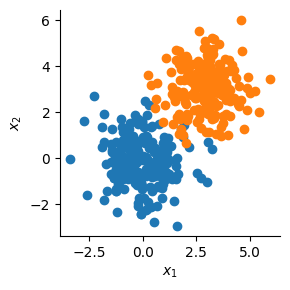
\includegraphics[scale=0.8, max width=\linewidth]{./fig/local-learning-rule/logistic-regression-perceptron/cell006.png}
	\caption{cell006.png}
	\label{cell006.png}
\end{figure}
\lstinputlisting[language=julia]{./text/local-learning-rule/logistic-regression-perceptron/007.jl}
\lstinputlisting[language=julia]{./text/local-learning-rule/logistic-regression-perceptron/008.jl}
\lstinputlisting[language=julia]{./text/local-learning-rule/logistic-regression-perceptron/009.jl}
\begin{figure}[ht]
	\centering
	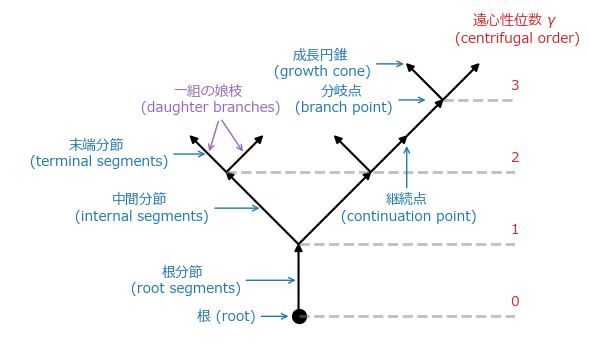
\includegraphics[scale=0.8, max width=\linewidth]{./fig/neuron-model/neurite-growth-model/cell009.png}
	\caption{cell009.png}
	\label{cell009.png}
\end{figure}
Here σ denotes the (point-wise) activation function, $W \in R^{m\times n}$
is the weight-matrix and $b \in R^n$
is
the bias-vector. The vector $x \in R^m$ and the vector $y \in R^n$ denote the input, respectively the output


\begin{equation}
y=\sigma(W^\top x + b)
\end{equation}



\begin{align}
& \text { Initialize } W^0, b^0 \text {; } \\
& \text { for } k=1,2, \ldots \text { do } \\
& \qquad \begin{array}{|l}
\text { for } i=1, \ldots, s \text { do } \\
e_i=y_i-\sigma\left(\left(W^k\right)^{\top} x_i+b^k\right) \\
W^{k+1}=W^k+e_i x_i^{\top} \\
b^{k+1}=b^k+e_i
\end{array} \\
& \text { end }
\end{align}
\lstinputlisting[language=julia]{./text/local-learning-rule/logistic-regression-perceptron/011.jl}
\lstinputlisting[language=julia]{./text/local-learning-rule/logistic-regression-perceptron/012.jl}
\begin{figure}[ht]
	\centering
	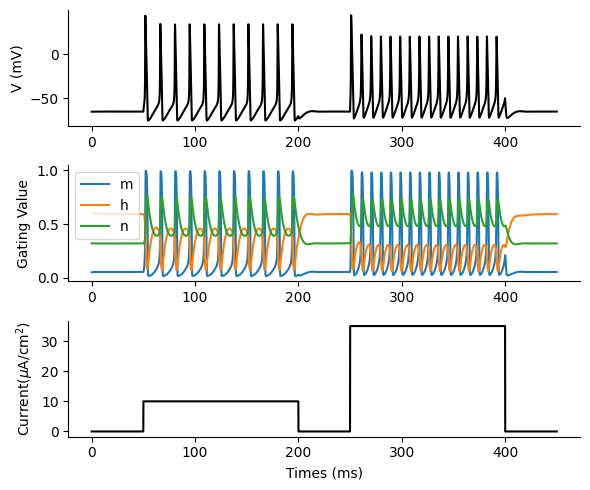
\includegraphics[scale=0.8, max width=\linewidth]{./fig/neuron-model/hodgkin-huxley/cell012.png}
	\caption{cell012.png}
	\label{cell012.png}
\end{figure}
\lstinputlisting[language=julia]{./text/local-learning-rule/logistic-regression-perceptron/013.jl}
\lstinputlisting[language=julia]{./text/local-learning-rule/logistic-regression-perceptron/014.jl}
ax + by + c = 0  
y = -a/b x - c/b
\lstinputlisting[language=julia]{./text/local-learning-rule/logistic-regression-perceptron/016.jl}
\lstinputlisting[language=julia]{./text/local-learning-rule/logistic-regression-perceptron/017.jl}
\begin{figure}[ht]
	\centering
	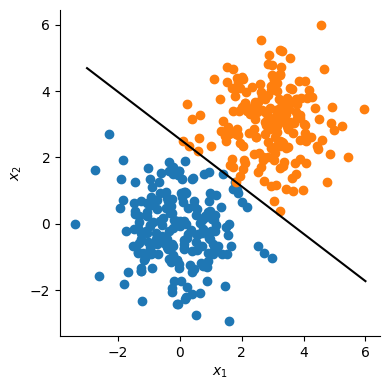
\includegraphics[scale=0.8, max width=\linewidth]{./fig/local-learning-rule/logistic-regression-perceptron/cell017.png}
	\caption{cell017.png}
	\label{cell017.png}
\end{figure}
